%==========================================================================
\section{Discussion}
\label{sec:disc}
\textbf{Which coverage to trust.}
Two coverage numbers come out of the same calibration.
Theorem~\ref{thm:cov} certifies
\emph{simultaneous} coverage, and that is exactly the quantity the
seen-to-unseen move pulls below target ($0.82$ to $0.89$ at $\alpha=0.10$),
while \emph{step-averaged} coverage is what the runs verify above $1-\alpha$
(Section~\ref{ssec:gap}). The gap has one door, the exchangeability
premise, and it obeys an inequality: coverage is one event in the joint
episode law, so $\dtv(P,Q)\leq\delta$ implies simultaneous coverage under
$Q$ of at least $1-\alpha-\delta$ (cf.~\cite{barber2023beyond}). We
estimate the shift with a plug-in total
variation between the two score laws, $\dtv = 0.156$, a $50$-bin histogram
of the THR teacher score $1-p_{\mathrm{teacher}}$ that is stable across bin
counts. Because this is a \emph{marginal} of the episode
record, it lower-bounds $\delta$, so it certifies that the premise is broken
rather than that the loss is small; the observed $0.82$ to $0.89$ is
consistent with the bound at $\delta \geq 0.156$
($1-\alpha-\delta \leq 0.744$). Binning $|\mathcal{A}_t|$ instead gives
$0.070$, so most of the movement is appearance change rather than branching
factor. The practical reading is to act on the step-level coverage the runs
verify and recalibrate inside each new building, which restores the premise
and the guarantee with it (Remark~\ref{rem:premise}).

\textbf{When the set fills the corridor.}
Rearranging the membership test $\snorm\leq\hat q$ for THR gives a
deterministic saturation condition: $C_\alpha(x_t)=\mathcal{A}_t$ only when
$\hat q\geq(1-\min_a p_a)/(2-\pmax)\geq(1-1/|\mathcal{A}_t|)/(2-\pmax)$, so a
small $|\mathcal{A}_t|$ makes saturation possible. At the DUET-full median
step ($|\mathcal{A}_t|\!\approx\!8$, $\pmax\!\approx\!0.80$) the right-hand
side is $0.73$, below the calibrated $\hat q$, and the same holds on every
backbone. The sets are small in absolute terms (mean $4$ to $7$), but the
action spaces are small too, and the saturation rate, the fraction of steps
whose set spans the whole action space, is $62$ to $83\%$ at $\alpha = 0.10$.
A robot in a narrow corridor will often see a set that spans every exit, the
operational cost of a divisive form that can only widen; a score that can also
tighten easy steps is left for future work.

\textbf{One episode, step by step.}
Figure~\ref{fig:qualitative} walks through one val-unseen DUET-full episode
at the deployed threshold ($\hat q = 0.989$, THR, $\alpha=0.10$). For two steps the policy is certain and the set is a
singleton; from step~$2$ the instruction stops matching what the agent sees,
$\pmax$ falls to $0.20$--$0.31$, the top action is wrong on five of the six
remaining steps, and the set widens until it holds the teacher at each.
Help is summoned precisely where the policy is about to err, at the
cost of a set that spans the whole frontier. The set flags \emph{that} the
agent is lost, not \emph{which} exits to prefer.

\begin{figure}[t]
\centering
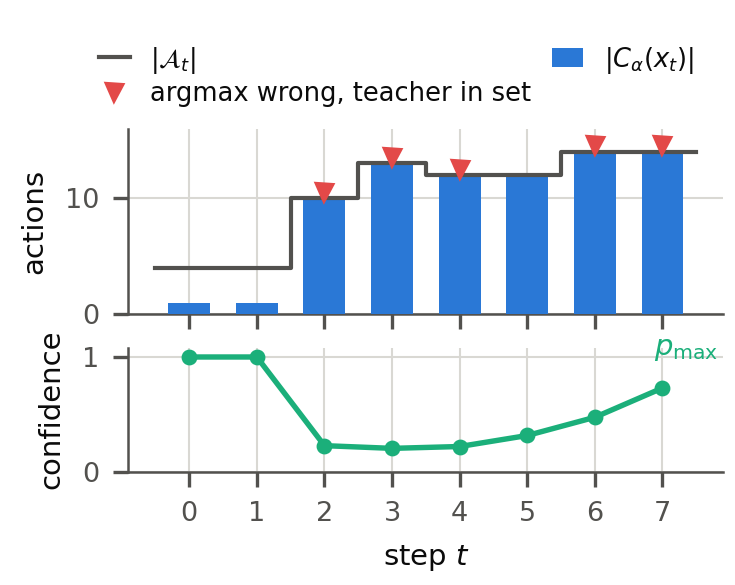
\includegraphics[width=0.63\linewidth]{figures/fig_qualitative.png}
\caption{A single val-unseen episode (DUET-full, THR, $\alpha=0.10$). Top:
prediction-set sizes (bars), the action-space size $|\mathcal{A}_t|$
(staircase), and triangles marking steps where the policy's top action is
wrong but the teacher action stays inside the set. Bottom: the policy
confidence $\pmax$.}
\label{fig:qualitative}
\end{figure}

\textbf{The momentum of an early mistake.}
An early misread correlates every later step, and under step-pooled
calibration this dependence is what voids the guarantee. The episode-maximum
unit dissolves the problem instead of pricing it, since
Theorem~\ref{thm:cov} lets steps depend arbitrarily when only whole
episodes are compared. Episodes themselves cluster (several instructions
per path, several paths per building), which shrinks the effective sample
behind $n=1021$; the scan-cluster intervals of Section~\ref{ssec:main}
price this in, and exact ties in the episode maxima (fp16 logits) affect at
most $2.3\%$ of calibration episodes, pushing coverage up, never down.

\textbf{A learned weight works too.}
Table~\ref{tab:learned} evaluates the weight family of
Section~\ref{ssec:learned} on R2R DUET-full at $\alpha=0.10$. The learned
member stacks the softmax entropy, $\pmax$, the top-two margin,
$\log|\mathcal{A}_t|$, the normalised step index, and $\alpha$ into
$\phi(x_t)$ and trains $w_\psi$ to predict the difficulty ratio
$(1-p_{\mathrm{teacher}})/(1-\pmax)$ on half of calibration. Every member
holds the target coverage; the learned and combined weights do so at
slightly larger sets, and the combined member matches the parameter-free
coverage to three decimals, so the learned residual adds little once the
confidence floor is in place. The feature set is not what carries the
effect. With all weights calibrated on the same held-out half, learned and
parameter-free coverage differ by at most $0.009$ on every backbone and on
both REVERIE agents, dropping the $\alpha$ feature leaves coverage at
$0.974$, and even a frozen random MLP stays above target at $0.982$, so
\emph{any} positive scale restores the response to $\alpha$; what earns
$1-\pmax$ its place is that it needs no tuning and its threshold transfers
(Section~\ref{ssec:gap}). The parameter-free score is the one we carry to
REVERIE.

\begin{table}[t]
\centering
\caption{Parameter-free versus learned per-step scale $g(x_t)=1+w(x_t)$ (R2R
DUET-full, THR, $\alpha=0.10$).}
\label{tab:learned}
\setlength{\tabcolsep}{4pt}\footnotesize
\begin{tabular}{lccc}
\toprule
Per-step weight $w(x_t)$ & cov & $\overline{|C|}$ & trained? \\
\midrule
$w=0$ (no normalisation)              & 0.967 & 4.7 & no \\
$w=1-\pmax$ (parameter-free)          & 0.968 & 6.8 & no \\
$w=w_\psi(\phi(x_t))$ (learned MLP)   & 0.974 & 7.6 & \textbf{yes} \\
\quad learned, without $\alpha$ feature & 0.974 & 7.5 & \textbf{yes} \\
$w=(1-\pmax)+r_\psi(\phi(x_t))$ (combined) & 0.968 & 7.3 & \textbf{yes} \\
$w=$ frozen random MLP                & 0.982 & 7.0 & no \\
\bottomrule
\end{tabular}
\end{table}


\textbf{Generalisation to REVERIE.}
Beyond R2R we run the method on REVERIE~\cite{qi2020reverie}, a
remote-object-grounding task, with the DUET and HAMT agents (reproduced
val-unseen success $45.9$ against $47.0$ and $33.9$ against $33.0$).
First, the step-level guarantee holds on both agents, with coverage clearing
the target in every $\alpha$ cell (Table~\ref{tab:reverie},
Figure~\ref{fig:reverie}), and saturation stays high ($0.90$ on DUET, $0.94$
on HAMT at $\alpha=0.10$, against $0.70$ on R2R); by the saturation condition
above this traces to the confidence law and the threshold rather than to
action-space size. Second, we conformalise the object-grounding head, a
single classification per episode under plain split CP. There the same
normalisation does not restore coverage, because the grounder is both
concentrated and strongly shifted seen-to-unseen; coverage falls to $0.80$
on DUET and $0.90$ on HAMT at $\alpha=0.10$, a drop that sits on the broken
exchangeability premise. Calibrating on a
split of the deployment distribution returns coverage to its target in every
case we tested (navigation and grounding, DUET and HAMT, R2R and REVERIE),
which confirms that the drop is covariate shift and that no learned or
weighted score is needed for validity.

\begin{figure}[!ht]
\centering
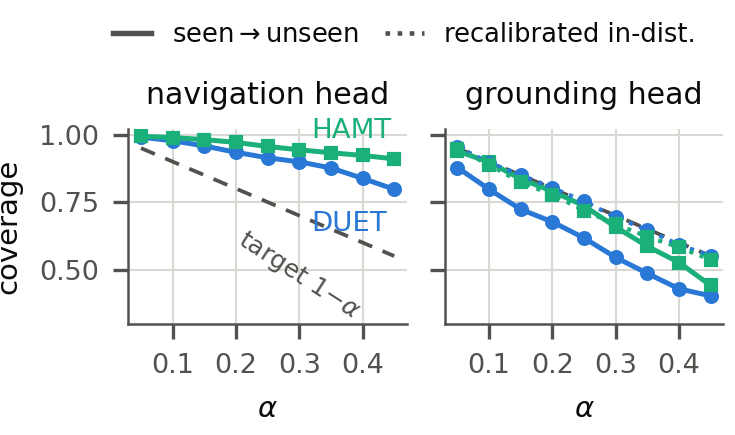
\includegraphics[width=0.63\linewidth]{figures/fig_reverie.png}
\caption{The REVERIE object-grounding head undercovers at every level under
the seen-to-unseen shift, which in-distribution recalibration restores;
navigation coverage on REVERIE clears its target (Table~\ref{tab:reverie}).}
\label{fig:reverie}
\end{figure}

\begin{table}[t]
\centering
\caption{Zero-Shot Normalised CP on REVERIE val-unseen (navigation head), on
the two agents with public REVERIE checkpoints; APS matches THR to within
$0.002$ everywhere and is omitted.}
\label{tab:reverie}
\setlength{\tabcolsep}{2.6pt}\scriptsize
\begin{tabular}{ll ccc c ccc c ccc}
\toprule
& & \multicolumn{3}{c}{$\alpha{=}0.10$} & &
    \multicolumn{3}{c}{$\alpha{=}0.20$} & &
    \multicolumn{3}{c}{$\alpha{=}0.30$} \\
\cmidrule{3-5}\cmidrule{7-9}\cmidrule{11-13}
\textbf{Backb.} & \textbf{Sc.}
 & cov & $\overline{|C|}$ & sat & & cov & $\overline{|C|}$ & sat
 & & cov & $\overline{|C|}$ & sat \\
\midrule
\multirow{2}{*}{DUET}
 & THR  & .977 & 8.8 & .90 & & .935 & 8.2 & .79 & & .899 & 7.6 & .70 \\
 & RAPS & .965 & 7.1 & .50 & & .893 & 5.2 & .20 & & .808 & 4.1 & .09 \\
\midrule
\multirow{2}{*}{HAMT}
 & THR  & .989 & 5.3 & .94 & & .971 & 5.0 & .87 & & .944 & 4.7 & .78 \\
 & RAPS & .991 & 5.3 & .91 & & .978 & 5.0 & .80 & & .965 & 4.8 & .73 \\
\bottomrule
\end{tabular}
\end{table}


\textbf{Conditional coverage.}
The episode-maximum unit alone, with $w=0$, already gives step coverage
$0.967$ at $\overline{|C|}=4.7$ on DUET-full, so normalisation buys the
response to $\alpha$ at the price of larger sets. Coverage by $\pmax$
quartile, least to most confident, is $1.00$, $1.00$, $0.97$, $0.90$: the
shortfall sits on the most-confident quartile, where the set is a singleton
and a confident wrong step is missed; by action-space-size class it is near
uniform ($0.96$--$0.97$).

\textbf{Acting on the sets.}
Figure~\ref{fig:closedloop} closes the loop on DUET-full. A simulated
operator supplies the correct next action whenever a trigger fires, and we
sweep both triggers over val-unseen at the deployed threshold. Answering the
steps whose set exceeds $\tau$ converts modest attention into large gains,
with success rising from $71.2$ to $91.2$ when $32\%$ of steps are answered
($\tau=8$) and to $98.0$ at $57\%$ ($\tau=4$). A tuned confidence cutoff is
slightly stronger at a matched budget on this backbone ($95.0$ at $34\%$),
but the cutoff is an uncalibrated knob on a confidence
scale that shifts from $0.71$ to $0.84$ across our backbones, while the set
trigger inherits its operating point from $\alpha$ with a coverage
certificate and a threshold that transfers (Section~\ref{ssec:gap}).
Because saturated sets tie at the frontier size, the set trigger moves in
coarse jumps of $\tau$. The membership test itself costs under
$0.1$ ms per step on CPU, so the loop adds no perceptible latency.

\begin{figure}[!ht]
\centering
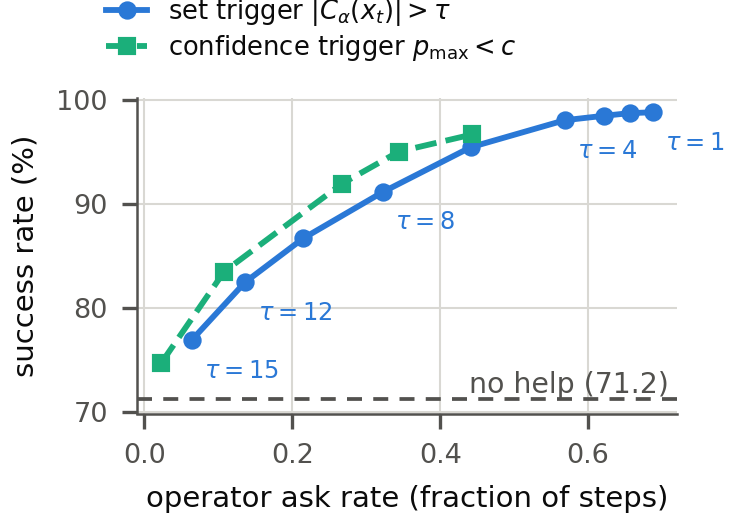
\includegraphics[width=0.63\linewidth]{figures/fig_closedloop.png}
\caption{Closing the loop (DUET-full, val-unseen, THR, $\alpha=0.10$). A
simulated operator answers a step when the trigger fires; success rate is
plotted against the fraction of steps answered, for the prediction-set
trigger $|C_\alpha|>\tau$ and the confidence trigger $\pmax<c$.}
\label{fig:closedloop}
\end{figure}

\textbf{What the standard remedies buy.}
Three canonical alternatives, run on the same rollouts, locate the method.
\emph{Temperature scaling} cannot restore the $\alpha$-response of the
adaptive scores, because a temperature preserves ranks and the top-ranked
APS score is exactly zero at any temperature, so whenever the calibration teacher sits
at rank one more often than $1-\alpha$, the collapse $\hat q=0$ survives the
best-fit temperature (DUET-full and HAMT still
return $100\%$ singletons at $\alpha=0.30$). \emph{Weighted CP} with a
logistic-regression density ratio over episode covariates targets the
simultaneous coverage the shift destroys and partially recovers it (HAMT
$0.83\to0.91$ at $\alpha=0.10$),
at the price of an estimated ratio and a reduced effective sample.
\emph{Mondrian calibration} by action-space class shrinks sets sharply
($1.1$ against $2.7$ on the small-degree class of DUET-full) but its
step-pooled quantiles undercover under the same shift and dependence ($0.78$
to $0.89$). Only recalibration inside the deployment distribution restores
the guarantee outright.

\textbf{Limitations.}
The whole-trajectory guarantee holds under exchangeable episodes and degrades
under the seen-to-unseen shift, which we measure and bound one-sidedly rather
than remove. Because the divisive form can only widen, the sets often span
the whole small action space (saturation up to $83\%$ at $\alpha = 0.10$ on
R2R and up to $94\%$ on REVERIE) and carry little resolution there. On the
object-grounding head the shift requires in-distribution recalibration to
keep the guarantee. The closed loop of Figure~\ref{fig:closedloop} simulates
the operator with the shortest-path teacher; a human-operator study is
future work.

\textbf{Beyond the discrete graph.}
Everything here lives on Matterport3D's discrete panoramic action space,
whose graph supplies the finite candidate set CP thresholds at every
step. Continuous instruction following, in
VLN-CE~\cite{krantz2020vlnce} or under velocity- or waypoint-level control
on a real platform, removes that finite set and with it every
classification score in this paper. The episode-maximum reduction, however,
does not care how the step is represented. Any fixed per-step score, including a conformal
\emph{regression} interval over a proposed waypoint or heading, reduces to
one exchangeable scalar per episode, and Theorem~\ref{thm:cov} applies
unchanged. Carrying the confidence-normalised family to waypoint heads in
continuous environments is the most promising direction this work opens.
